\documentclass{article}
\usepackage[UTF8]{ctex} % Required for inserting images
\usepackage{graphicx}
\usepackage{amsmath}

\title{机器学习}
\author{徐闻璐}
\date{2025 秋季学期}

\begin{document}
\maketitle

\newpage

\section{作业一}

    \begin{figure}[!h]
        \centering
        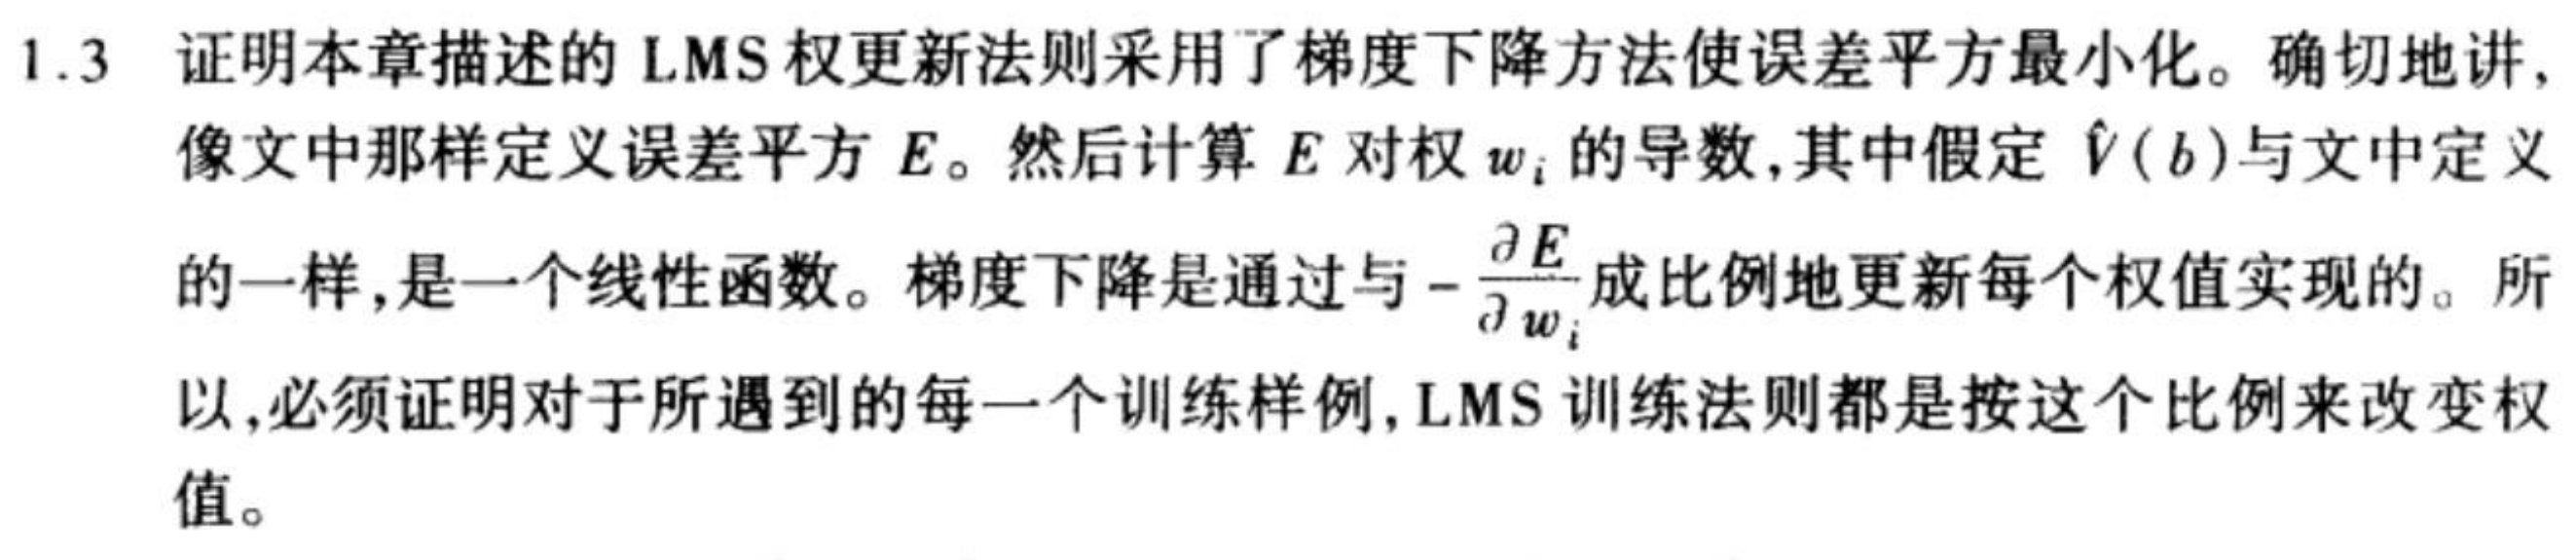
\includegraphics[width=1.2\linewidth]{image/1.3.jpg}
        \label{1.3}
    \end{figure}
        
\paragraph{证明:}
    定义误差平方$E$,第$i$个特征值对应的权为$w_{i}$。假定估计值函数$\hat{V}(b)$为线性函数。

    梯度下降是通过与$-\frac{\partial E}{\partial w_{i}}$成比例地更新每个权值实现的。
    
    要证明LMS权更新法采用了梯度下降法使误差平方最小化,必须证明对于所遇到的每一个训练样例,LMS训练法则都是按这个比例来改变权值的。

    对于单个训练样例$b$,定义误差平方函数为$E=\frac{1}{2}(V(b)-\hat{V}(b))^{2}$。

    其中$V(b)$为目标值,$\hat{V}(b)$为估计值。系数$\frac{1}{2}$简化导数计算,不影响法则本质。

    估计值$\hat{V}(b)=\sum_{i}w_ix_i(b)$是线性函数。

    其中$x_i(b)$是样例$b$的特征值。

    求偏导:$$\frac{\partial E}{\partial w_i}=\frac{\partial \frac{1}{2}(V(b)-\hat{V}(b))^2}{\partial w_i}$$

    令$e=V(b)-\hat{V}(b)=V(b)-\sum_jw_jx_j(b)$,则$E=\frac{1}{2}e^2$。

    由链式法则:
    $$\frac{\partial E}{\partial w_i}=\frac{\partial E}{\partial e}\cdot \frac{\partial e}{\partial w_i}=e\cdot \left(-\frac{\partial \hat{V}(b)}{\partial w_i}\right)$$

    由于$frac{\partial \hat{V}(b)}{\partial w_i}=x_i(b)$,有:
    $$\frac{\partial e}{\partial w_i}=-x_i(b)$$

    因此:
    $$\frac{\partial E}{\partial w_i}=e\cdot(-x_i(b))=-\left(V(b)-\hat{V}(b)\right)x_i(b)$$

    由于$\frac{\partial \hat{V}(b)}{\partial w_i}=x_i(b)$,有:
    $$\frac{\partial e}{\partial w_i}=-x_i(b)$$

    因此:
    $$\frac{\partial E}{\partial w_i}=e\cdot(-x_i(b))=-\left(V(b)-\hat{V}(b)\right)x_i(b)$$

    梯度下降法通过沿负梯度方向更新权值来最小化$E$。更新规则为:
    $$\Delta w_i=-\eta \frac{\partial E}{\partial w_i}$$

    其中$\eta$是学习率。代入上述导数:

    $$\Delta w_i=-\eta \left[-\left(V(b)-\hat{V}(b)\right)x_i(b)\right]=\eta \left(V(b)-\hat{V}(b)\right)x_i(b)$$

    因此,权值更新为:
    $$w_i\leftarrow w_i+\Delta w_i=w_i+\eta \left(V(b)-\hat{V}(b)\right)x_i(b)$$

    从而证明了LMS训练法则对于每一个训练样例的权值更新规则。也就是采用了梯度下降法,通过每次与$-\frac{\partial E}{\partial w_i}$成比例地更新权值,使误差平方最小化。

\end{document}
